\documentclass[12pt, a4paper]{article}

\usepackage{setspace, graphicx, lineno, caption, color, float}
\usepackage{amsmath}
\usepackage{amsfonts}
\usepackage{amssymb}
\usepackage{amsthm}
\usepackage{amstext} %to enter text in mathematical formulae
\usepackage[retainorgcmds]{IEEEtrantools}
\usepackage{natbib}
\usepackage{hyperref} % for linking refferences to supps
\usepackage{multirow} %connecting columns in tables
\usepackage{multicol}
\usepackage{longtable}
\usepackage{makecell}

%page set up
\usepackage[left=2.5cm,top=2.5cm,right=2.5cm, bottom=2.5cm,nohead]{geometry}

%paragraph formatting
\setlength{\parskip}{12pt}
\setlength{\parindent}{0cm}

\setcounter{figure}{0}
\renewcommand{\thefigure}{S\arabic{figure}}
\setcounter{table}{0}
\renewcommand{\thetable}{S\arabic{table}}

\begin{document}
\section*{Appendix 2: Finding which initial conditions and model parameters lead to which IPM strategies}
It is unlikely a given IPM strategy will perform well in all scenarios, for example strategy that works well in cases where the yield penalty ($Y_D$) of the weed is very low is unlikely to be good in cases where the yield penalty is very high. To find the parameters and initial conditions ($n_0$) that most influence what makes a good IPM strategy we extend the meta-modelling approach outlined in \citep{Cout2014} to complex multivariate time series outputs (i.e. the sequences of the four sub actions). The meta-modelling approach to global sensitivity analysis is very flexible, and only requires building a function that predicts a models output given a set of parameters. The complication in this case is that the model output is a time series of actions, rather than a single number. To address this use multi-variate boosted regression trees\citep{Mill2016} as follows:
\begin{enumerate}
\item We use latin hypercube sampling to generate 15000 parameter combinations, see Table \ref{tab:pars} for upper and lower limits of each parameter. We treat the initial conditions as parameters ($Rr_\text{int}$, $Qq_\text{int}$ and $N_\text{int}$). 
\item For each parameter combination we run the genetic algorithm (Appendix 1) for 100 iterations, experience showed that improvements to the best solution found dramatically slowed down after 60 iterations with a solution set size of 1000 and mutation rate or 0.03. After 100 iterations we choose the action sequence with the highest reward as the best action sequence.     
\item This resulted in 15000 action sequences. We only use the first 10 time steps of each action sequence, although the reward was calculated over 25 time steps. This ensured that the action chosen at each time step was done so considering rewards from at least 15 time steps in to the future. 
\item To make sense of this mass of data we built a dissimilarity matrix of each action sequence to all the other action sequences, to represent how all the action sequences related to each other. We use a distance metric from text analysis, longest common sub-sequence, calculated with the 'SimilarityMeasures' \citep{Tooh2015} package in R. We allow a positional displacement of one time step, that is actions in sequence A are allowed to be matched to actions in sequence B that are separated in time by at most one time step. This allows out of phase cycles to have very high similarity. Two action sequences where the same combinations of actions are used, but at times more than one tim step apart will have low similarity. 
\item We use non-metric multi-dimensional scaling (NMDS), implemented with the 'ecodist' package \citep{Gosl2007}, to project this very high dimensional dissimilarity matrix into a lower dimensional space. We call this the solution space and we found that we could project the dissimilarity matrix into an eight dimensional solution space, with a stress of 0.09. Stress measures the difference between the relative location of each solution in the solution space, and the dissimilarity matrix. Lower values are better. We found that 8 dimensions was a good trade-off between low stress and a manageable number of dimensions. Figure \ref{fig:clust_NMDS} shows how the solution space matches up to a separate hierarchical clustering (using the wardD2 method) we carried out to confirm and aid visualization of the NMDS.                  
\item We recorded the eight co-ordinates of each solution in the solution space, along with the parameter set that generated that solution. This built a data-set 15000 rows long, where each row was a parameter set and a location in the solution space.
\item We use multi-variate boosted regression trees (mvBRT) as our meta-model. mvBRTs were fit using the 'mvtboost' package \citep{Mill2016}. mvBRTs fit a separate boosted regression tree to each dimension of the response, in our case a position in the eight dimensional solution space. At each iteration in each tree the split that most reduced the co-variance between the eight responses is chosen. For further details see \citep{Mill2016}. We used a learning rate of 0.01, maximum interaction depth of 5. These tuning parameters lead to a optimum of 12229 trees in the mvBRT.
\item We interrogate the mvBRT to find the most influential parameters. We also calculate partial dependence plots of the mvBRT to predict where in the solution space a given set of parameters leads to, and use the closest solution to that location to estimate what a solution in the predicted location would look like. We use this as guide to help us explore and and interrogate the complex solution space. However, we have access to the data generating process and so do not need to rely on this estimate. For the actual plots in the results we re-run the genetic algorithm with the desired parameter combinations.                  
\end{enumerate}       

\begin{figure}[!h]
	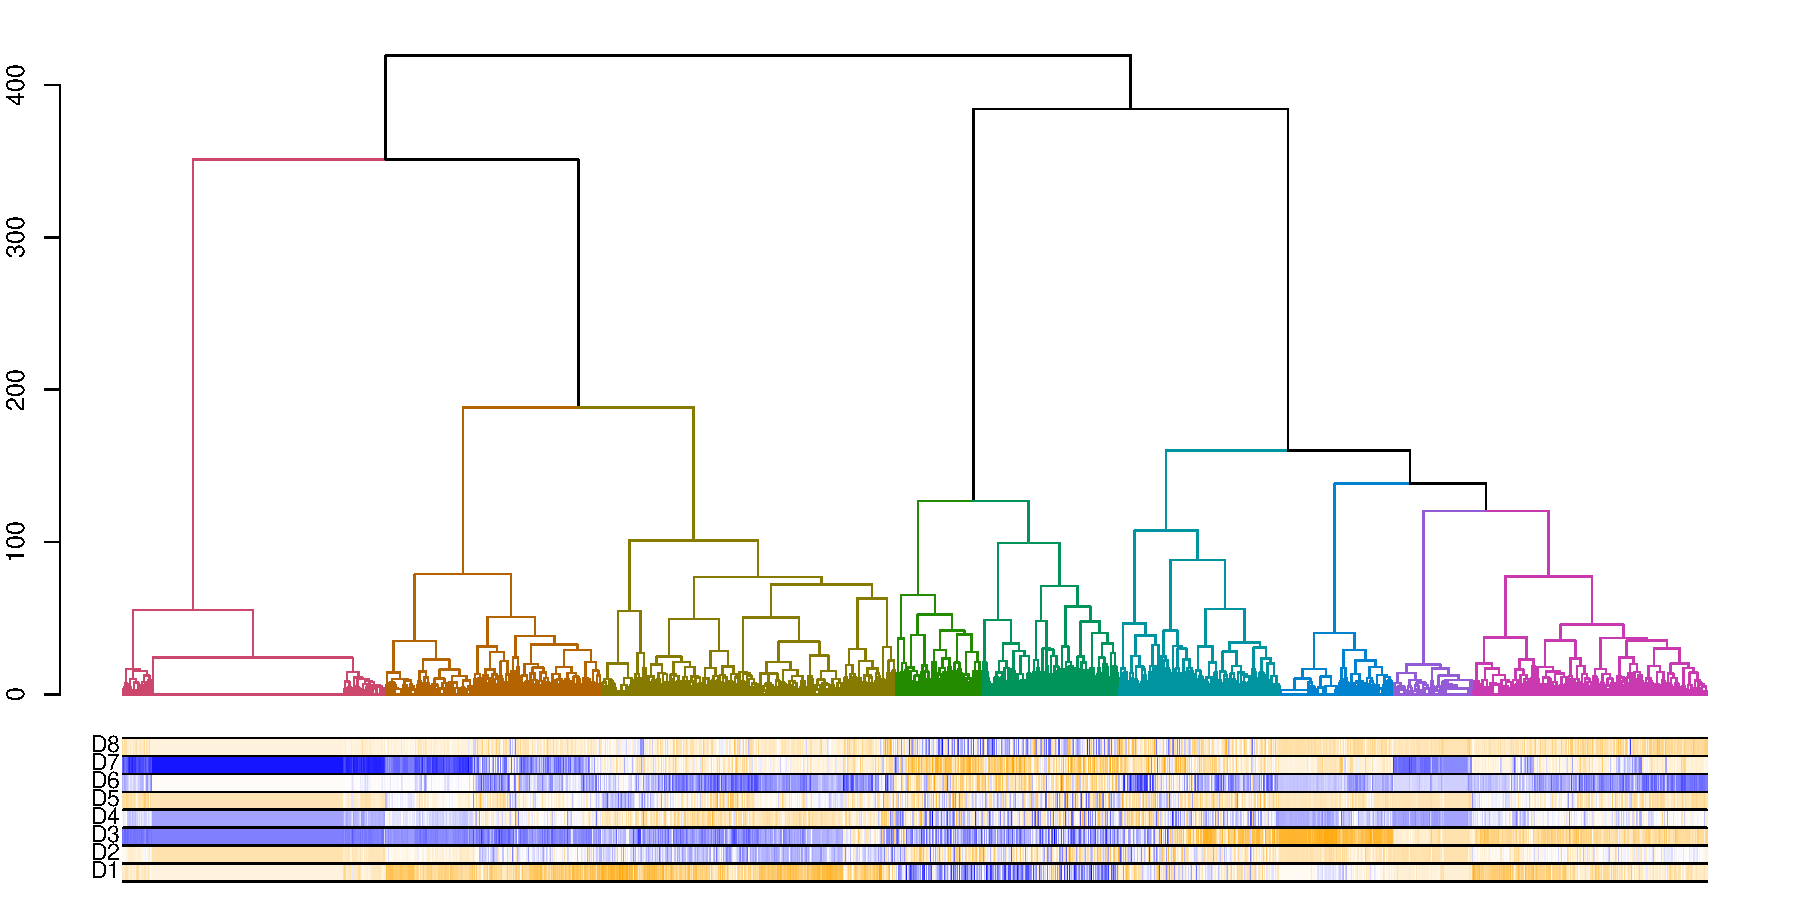
\includegraphics[width=170mm]{MS_figs/dend_9clust_NMDS_8D.pdf}
	\caption{Position of all 15000 IPM strategies found by the genetic algorithm in the eight dimensional solution space and dendrogram built using the wardD2 method. Different colors in the dendrogram highlight the 9 most distinct clusters. Colors in the bars show each solutions position in the solution space. All dimensions are centered on 0 (white), with dark blues being at one extreme and dark oranges the other (only relative position is meaningful).} 
	\label{fig:clust_NMDS}
\end{figure}

\newpage 

% table of parameters and ranges used
\begin{longtable}{c c c p{5cm} p{4cm}}
	\caption{Parameter descriptions and the range each parameter was tested over}
	\label{tab:pars}
	\\
	\hline
	\makecell{\textbf{Para-}\\\textbf{meter}} & \textbf{Units} & \textbf{Range} & \textbf{Description} & \textbf{Source} \\
	\hline
	\endhead
	\multicolumn{5}{l}{\textit{Population Model see Appendix 5}}\\
	$\phi_e$ & prob. & 0.45--0.6 & germination probability & \citet{Colb2006} \\ 
	$\phi_b$ & prob. & 0.2--0.86 & Probability a seed survives one year & \citet{Colb2006}, \citet{Thom1997}, \citet{Cava1999}\\
	$s_0$ & prob. & fixed 0.99 & Survival probability without herbicide & Assumed fixed and high so density effects only expressed through fecundity.\\
	$\theta$ & prob. & 0.7--1 & \multicolumn{2}{l}{\parbox[t]{9cm}{Proportion of \textit{A. myosuroides} population exposed to herbicide under sub-action $a_h$ = herb R, herb Q or both. plants may be missed spatially or temporally, or spraying may be affected by rain. Tested over wide range.}} \\       
	$s_h$ & prob. & 0.01 & Survival of susceptible \textit{A. myosuroides} exposed to herbicide ($a_h$ & herbicide assumed to be effective.\\
	$\alpha$ & prob. & 0.22--0.04 & Survival probability under the alternative crop ($a_k$ = alt), spring barley. & \citet{Lutm2013}\\
	$\beta$ & prob. & 0.05--0.2 & Survival under spot control (sub-action $a_s$), for example because plants are missed & tested over wide range.\\
	$f_m$ & \makecell[t]{seeds$\cdot$\\plant$^{-1}$} & 30--300 & \multicolumn{2}{l}{\multirow{2}{9cm}{\parbox[t]{9cm}{Number of seeds produced when density is 0 ($f_m$) and The effect of density on seed production ($f_d$) interact to determine maximum population size. Values chosen to keep the max population close to the maximum population seen in \citet{Quee2011} so yield is not extrapolated outside the observed range.}}} \\
	$f_d$ & $\frac{1}{plants\cdot ha^{-1}}$ & 0.001--0.0001 &  \\\\\\\\\\\\
	$I$ & prob. & 0.5--0.9 & The proportion of seed moved between seed bank levels by ploughing (sub-action $a_b$) & \citet{Grun1999} \\ 
	\multicolumn{5}{l}{\textit{Reward function see Appendix 3}}\\
	$\gamma$ & & 0.75--1 & discount rate on future returns & tested over wide range\\
	$Y_0$ & \pounds $\cdot ha^{-1}$ & 968--1758 & Yield from winter wheat when \textit{A. myosuroides} is absent. & Upper limit upper 95\% confidence interval from fitted yield function (Appendix 3). Lower limit from low production scenario \citet[pp.~9]{Nix2016}.\\
	$Y_D$ & \makecell[t]{\pounds$\cdot$plant$\cdot$\\$ha^{-1}$} & 0.0002--0.006 & reduction in yield caused by each \textit{A. myosuroides}. & 95\% confidence interval from fitted yield function, see Appendix 3. \\
	$\vartheta$ & \pounds$\cdot ha^{-1}$ & 672--920 & Yield of spring barley, an alternative crop commonly used to control \textit{A. myosuroides}. & \citet[pp.~12]{Nix2016}\\
	 $\varpi$ & prop. & 0.85--1 & proportion of yield achieved if crop $a_k$ is repeated & \citet[pp.~9]{Nix2016} \\
	 $\eta_h$ & \pounds$\cdot ha^{-1}$ & 50--100 & Cost of a single herbicide application & \citet[pp.~9]{Nix2016}\\
	 $\eta_b$ & \pounds$\cdot ha^{-1}$ & 55--92 & Cost of ploughing & \citet[pp.~202]{Nix2016}\\
	 $\eta_s^0$ & \pounds$\cdot ha^{-1}$ & 10--100 & Cost of spot control even when \textit{A. myosuroides} density is 0 & tested over wide range\\
	 $\eta_s$ & \makecell[t]{\pounds$\cdot$plant$\cdot$\\$ha^{-1}$} & 10--100 & Increase in spot control cost for each \textit{A. myosuroides} & tested over wide range\\
	 $\eta_\text{wheat}$ & \pounds$\cdot ha^{-1}$ & 383 & Cost of growing winter wheat not associated with \textit{A. myosuroides} control & \citet[pp.~9]{Nix2016}\\ 
	 $\eta_\text{alt}$ & \pounds$\cdot ha^{-1}$ & 273 & Cost of growing the alternative crop, spring barley. & \citet[pp.~12]{Nix2016}\\	    
	 $\eta_\text{fal}$ & \pounds$\cdot ha^{-1}$ & 36 & Cost of a fallow rotation. Based on two applications of glyphosate to control any germinating \textit{A. myosuroides}. &  \citet[pp.~202 and 284]{Nix2016}\\
	\multicolumn{5}{l}{\textit{Initial Conditions}}\\
	$R_\text{int}$ & & 0--1 & Initial frequency of R alleles & \\
	$Q_\text{int}$ & & 0--1 & Initial frequency of Q alleles & \\ 
	$N_\text{int}$ & & \makecell[t]{100--\\100000} & Initial number of seeds in each level of the seed bank & \\
	\hline
\end{longtable}

\section*{Appendices}
Appendix 1: Genetic Algorithm
Appendix 3: Reward Function
Appendix 5: Population Model

\bibliographystyle{/Users/shauncoutts/Dropbox/shauns_paper/referencing/bes}
\bibliography{/Users/shauncoutts/Dropbox/shauns_paper/referencing/refs} 

\end{document}
